%%%%%%%%%%%%%%%%%%%%%%%%%%%%%%%%%%%%%%%%%
% Jacobs Landscape Poster
% LaTeX Template
% Version 1.0 (29/03/13)
%
% Created by:
% Computational Physics and Biophysics Group, Jacobs University
% https://teamwork.jacobs-university.de:8443/confluence/display/CoPandBiG/LaTeX+Poster
% 
% Further modified by:
% Nathaniel Johnston (nathaniel@njohnston.ca)
%
% Modified further still by:
% Abraham Nunes (nunes <at> dal <dot> ca)
%
% License:
% CC BY-NC-SA 3.0 (http://creativecommons.org/licenses/by-nc-sa/3.0/)
%
%%%%%%%%%%%%%%%%%%%%%%%%%%%%%%%%%%%%%%%%%

%----------------------------------------------------------------------------------------
%	PACKAGES AND OTHER DOCUMENT CONFIGURATIONS
%----------------------------------------------------------------------------------------

\documentclass[final,table]{beamer}
\usepackage{multirow}

\usepackage[scale=1.24]{beamerposter} % Use the beamerposter package for laying out the poster
\usepackage{array}
\usetheme{confposter} % Use the confposter theme supplied with this template
\usepackage{bm}
\usepackage{xspace}
\usepackage{mathtools}
\usepackage{bm}
\usepackage{multirow}
\usepackage{adjustbox}
\setbeamercolor{block title}{fg=black,bg=} % Colors of the block titles
\setbeamercolor{block body}{fg=black,bg=} % Colors of the body of blocks
\setbeamercolor{block alerted title}{fg=white,bg=black} % Colors of the highlighted block titles
\setbeamercolor{block alerted body}{fg=black,bg=white} % Colors of the body of highlighted blocks
% Many more colors are available for use in beamerthemeconfposter.sty

\newcommand{\deemph}[1]{{\color{black!40}#1}}

%-----------------------------------------------------------
% Define the column widths and overall poster size
% To set effective sepwid, onecolwid and twocolwid values, first choose how many columns you want and how much separation you want between columns
% In this template, the separation width chosen is 0.024 of the paper width and a 4-column layout
% onecolwid should therefore be (1-(# of columns+1)*sepwid)/# of columns e.g. (1-(4+1)*0.024)/4 = 0.22
% Set twocolwid to be (2*onecolwid)+sepwid = 0.464
% Set threecolwid to be (3*onecolwid)+2*sepwid = 0.708

\newlength{\sepwid}
\newlength{\onecolwid}
\newlength{\twocolwid}
\newlength{\threecolwid}
\setlength{\paperwidth}{48in} % A0 width: 46.8in
\setlength{\paperheight}{36in} % A0 height: 33.1in
\setlength{\sepwid}{0.024\paperwidth} % Separation width (white space) between columns
\setlength{\onecolwid}{0.22\paperwidth} % Width of one column
\setlength{\twocolwid}{0.464\paperwidth} % Width of two columns
\setlength{\threecolwid}{0.708\paperwidth} % Width of three columns
\setlength{\topmargin}{-0.5in} % Reduce the top margin size

\makeatletter
\newcommand{\srcsize}{\@setfontsize{\srcsize}{5pt}{5pt}}
\makeatother

\setbeamerfont{bibliography entry author}{size=\tiny,}
\setbeamerfont{bibliography entry title}{size=\tiny}
\setbeamerfont{bibliography entry location}{size=\tiny,}
\setbeamerfont{bibliography entry note}{size=\tiny,}
%-----------------------------------------------------------

\usepackage{graphicx}  % Required for including images

\usepackage{booktabs} % Top and bottom rules for tables
\usepackage{setspace}
\DeclarePairedDelimiter\abs{\lvert}{\rvert}%
\DeclarePairedDelimiter\norm{\lVert}{\rVert}%
%----------------------------------------------------------------------------------------
%	TITLE SECTION 
%----------------------------------------------------------------------------------------

\title{Modeling Ants on Uneven Terrain} % Poster title

\author{Matthew Moreno$^{1}$, Jason Graham$^{2}$, Simon Garnier$^{3}$} % Author(s)

\institute{$^{1}$University of Puget Sound,
		   $^{2}$University of Scranton,
           $^{3}$New Jersey Institute of Technology }% Institution(s)

%----------------------------------------------------------------------------------------

\begin{document}
\addtobeamertemplate{block end}{}{\vspace*{2ex}} % White space under blocks
\addtobeamertemplate{block alerted end}{}{\vspace*{2ex}} % White space under highlighted (alert) blocks

\setlength{\belowcaptionskip}{2ex} % White space under figures
\setlength\belowdisplayshortskip{2ex} % White space under equations

\begin{frame}[t] % The whole poster is enclosed in one beamer frame

\begin{columns}[t] % The whole poster consists of three major columns, the second of which is split into two columns twice - the [t] option aligns each column's content to the top

\begin{column}{\sepwid}\end{column} % Empty spacer column

\begin{column}{\onecolwid} % The first column

%----------------------------------------------------------------------------------------
%	INTRODUCTION
%----------------------------------------------------------------------------------------
\vspace{-3.5ex}
\begin{block}{Summary}
\vspace{-2.5ex}
{\small
Ant foraging behavior is a collective decision making process in which, through  pheromone deposition and individual interactions between ants, a colony of ants selects and exploits a path between their nest and a food source. Research into the collective decision making strategies of ants, in addition to characterizing the biological mechanisms and emergent properties of the foraging process, has the potential to be leveraged into applications such as swarm robotics and commercial logistics management. Although ant foraging behavior has been extensively studied on flat terrains, ant foraging over uneven terrains is not well studied. This research presents an individual-based set of differential equations to model ant foraging behavior over uneven terrain in an enclosed arena. This model is employed to investigate the characteristics of foraging paths that ants tend towards when foraging over simple inclines of varying magnitudes. Numerical solutions of the model predict that, over most inclines, ants tend to favor the direct path between nest and food, with the direct path typically being more strongly favored when foraging over steep inclines.
}
\vspace{-0.5ex}
\begin{columns}[T, onlytextwidth]
\column{0.65\textwidth}
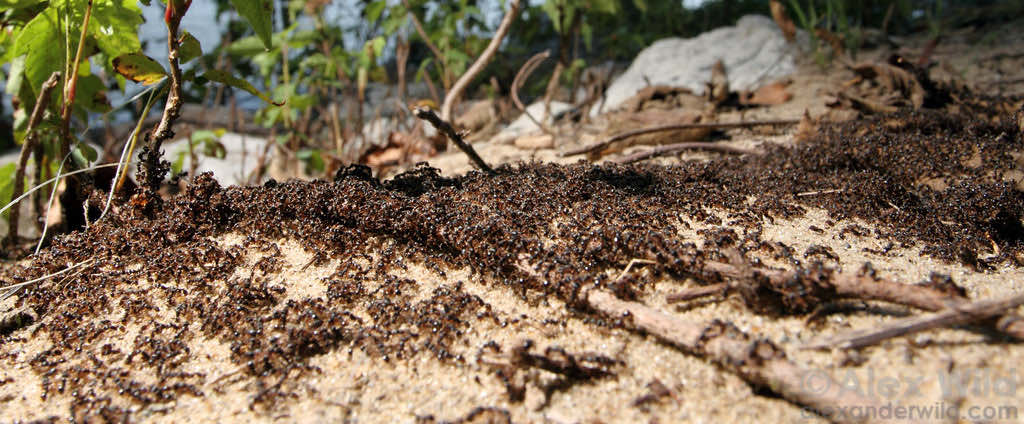
\includegraphics[width=\textwidth]{images/ant_battle1-XL_reduced}
\column{0.05\textwidth}
\column{0.3\textwidth}
\begin{spacing}{1.0}
{\small
\textit{Tetramorium caespitum} (Photo courtesy Alexander Wild.)}
\end{spacing}
\end{columns}

% Ant colonies, such as those of \textit{Lasius niger}, commonly employ foraging behavior to procure food. This process begins with individual ants exploring their environment nearly at random. Once an ant discovers a food source, it retrieves a load of food and returns to the nest. As the ant travels back towards the nest, it lays a pheromone trail for other ants to follow to the food source. As the foraging process continues, more ants proceed to the food source and, returning to the nest, lay their own pheromone. This process has several intriguing properties: ants tend take the shortest path to the food and they tend to select the richer food. \cite{camazine_self-organization_2003} 

% While ma
% This type of process is interesting because  ant conservation, swarm robotics, traffic management... potential applications

% The general approach to understanding is modeling and studies... past work... Although some effort has been put into understanding how individual ants behave in nonuniform elevation, the swarm dynamics of foraging ants has only been modeled on flat surfaces... Recent work (by Professor Garnier?) (?) has shown that ants in vivo tend select the least-energy path across uneven terrain from nest to food. The question of how they do this is unanswered. We set out to build a mathematical model to try to understand this phenomenon.
\end{block}

%------------------------------------------------

%----------------------------------------------------------------------------------------
%	OBJECTIVES
%----------------------------------------------------------------------------------------


%----------------------------------------------------------------------------------------

\end{column} % End of the first column

\begin{column}{\sepwid}\end{column} % Empty spacer column

\begin{column}{\twocolwid} % Begin a column which is two columns wide (column 2)

%----------------------------------------------------------------------------------------
%	IMPORTANT RESULT
%----------------------------------------------------------------------------------------

\vspace{-3.5ex}
\begin{block}{Model Components}
\vspace{-5ex}
\begin{tabular}{*{4}{>{\centering\arraybackslash}p{0.25\textwidth}}}
\begin{centering}
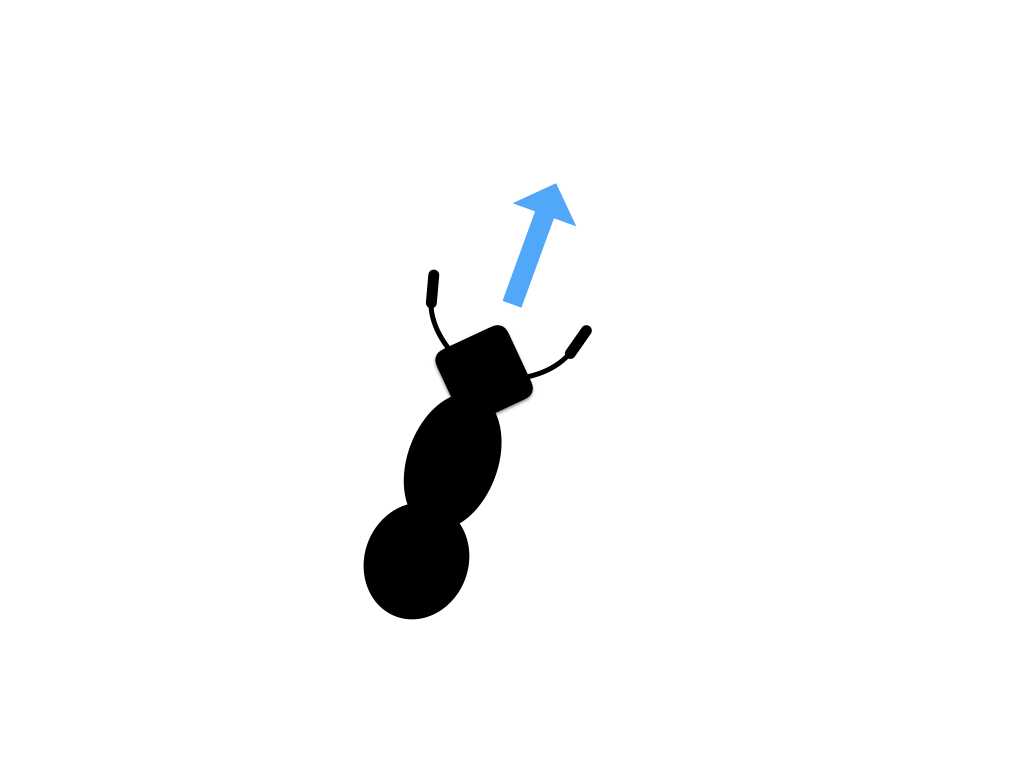
\includegraphics[width=0.20\textwidth]{images/model_components_cartoons_001}
\end{centering} &
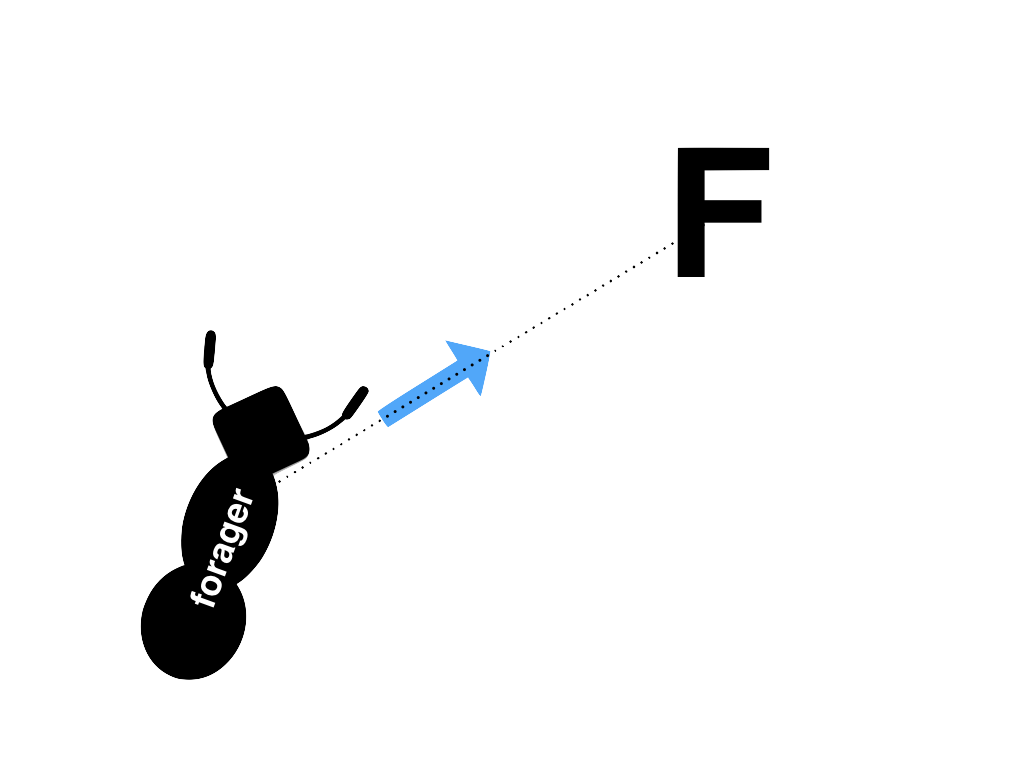
\includegraphics[width=0.20\textwidth]{images/model_components_cartoons_004} &
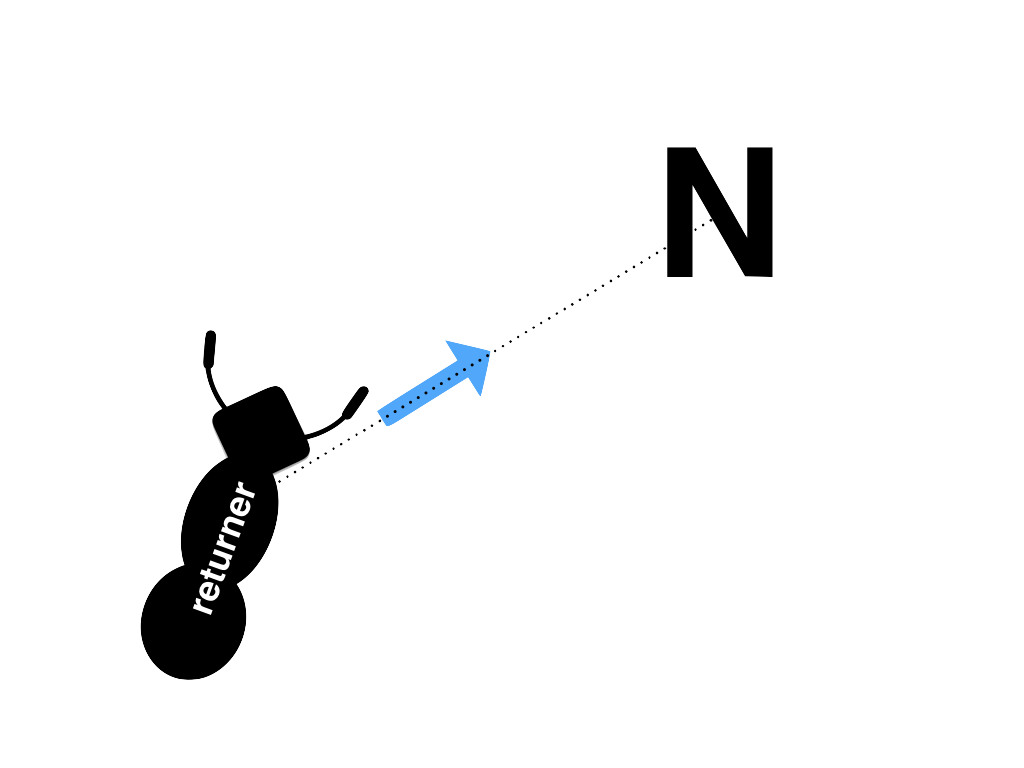
\includegraphics[width=0.20\textwidth]{images/model_components_cartoons_002} & 
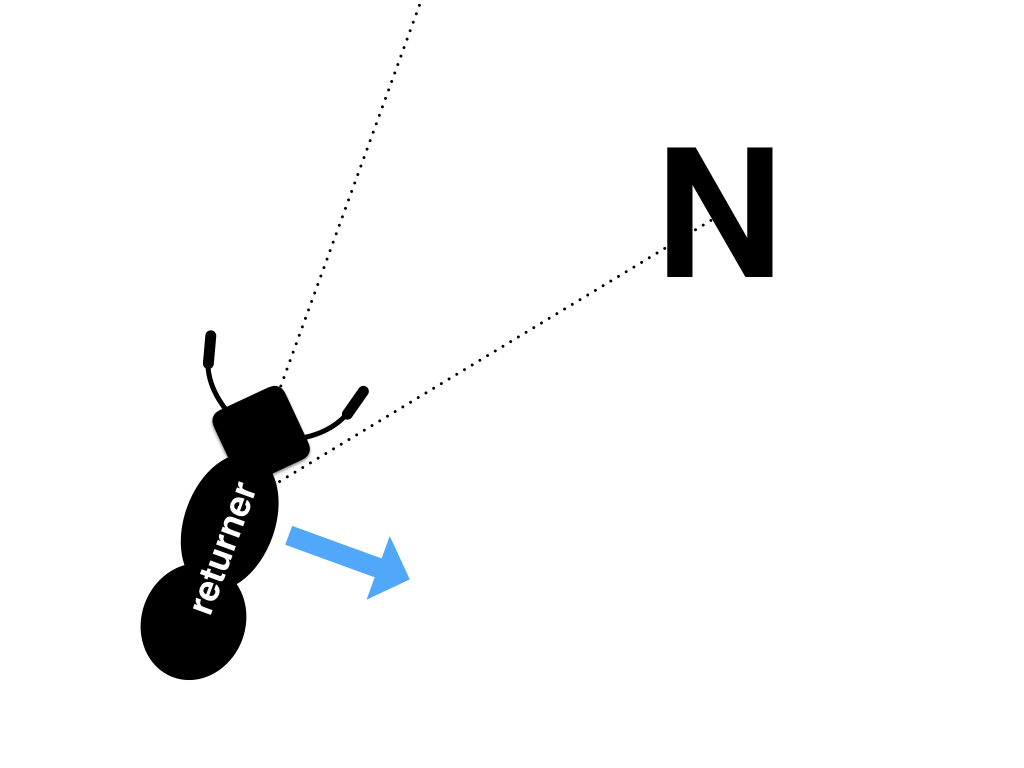
\includegraphics[width=0.20\textwidth]{images/model_components_cartoons_003} \\
\begin{spacing}{1.0}
\raggedright{\small
\textbf{Constant Power Propulsion} ants move fastest on slight decline}
\end{spacing} &
\begin{spacing}{1.0}
\raggedright{\small
\textbf{Food Attraction} magnitude increases exponentially with proximity to food}
\end{spacing} &
\begin{spacing}{1.0}
\raggedright{\small
\textbf{Nest Attraction} returner ant accelerates towards nest with constant magnitude}
\end{spacing} &
\begin{spacing}{1.0}
\raggedright{\small
\textbf{Near Nest Attraction} magnitude increases with nest proximity; acts $\perp$ to heading}
\end{spacing}
\\[-1.5cm]
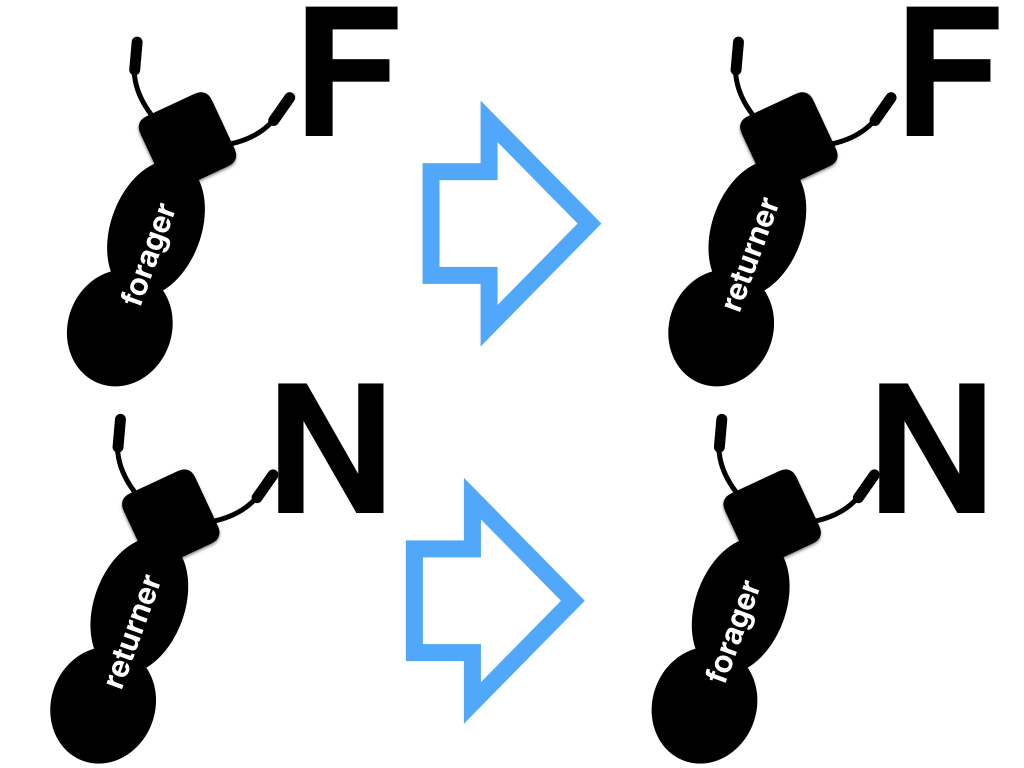
\includegraphics[width=0.20\textwidth]{images/model_components_cartoons_005} &
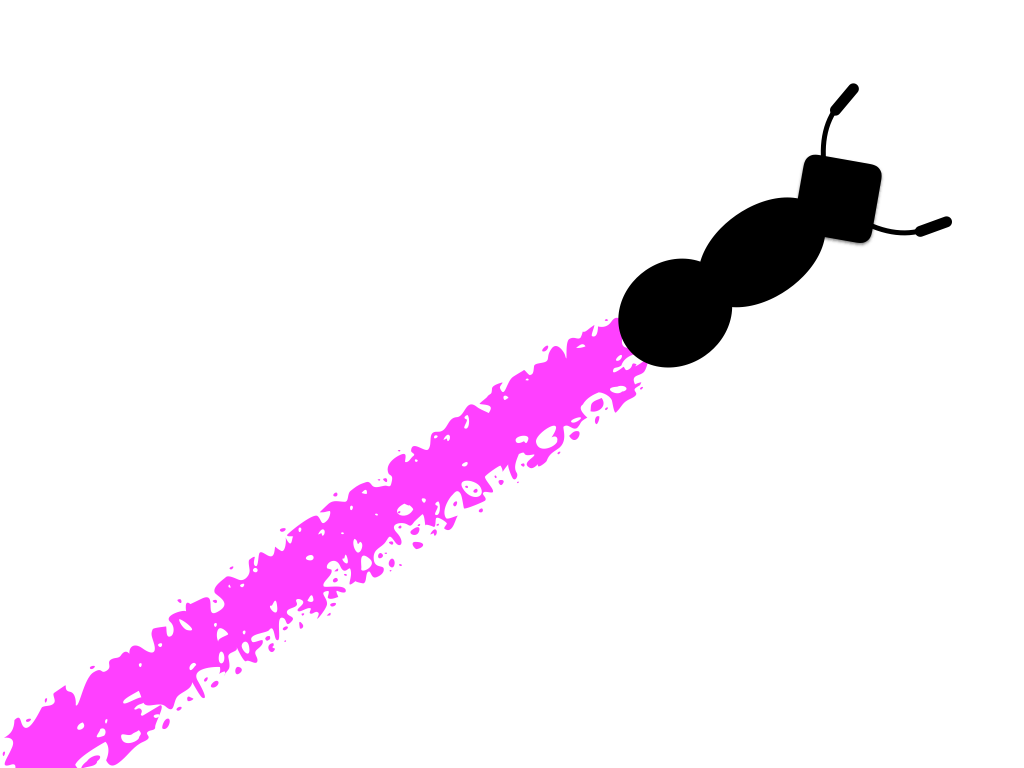
\includegraphics[width=0.20\textwidth]{images/model_components_cartoons_006} &
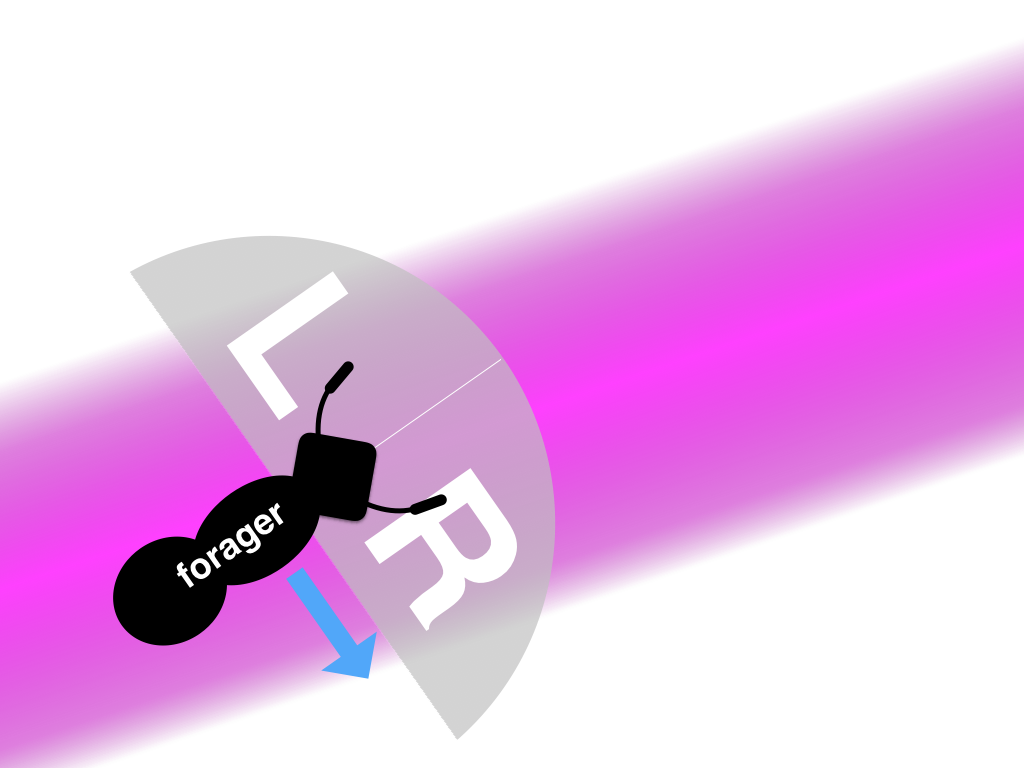
\includegraphics[width=0.20\textwidth]{images/model_components_cartoons_007} &
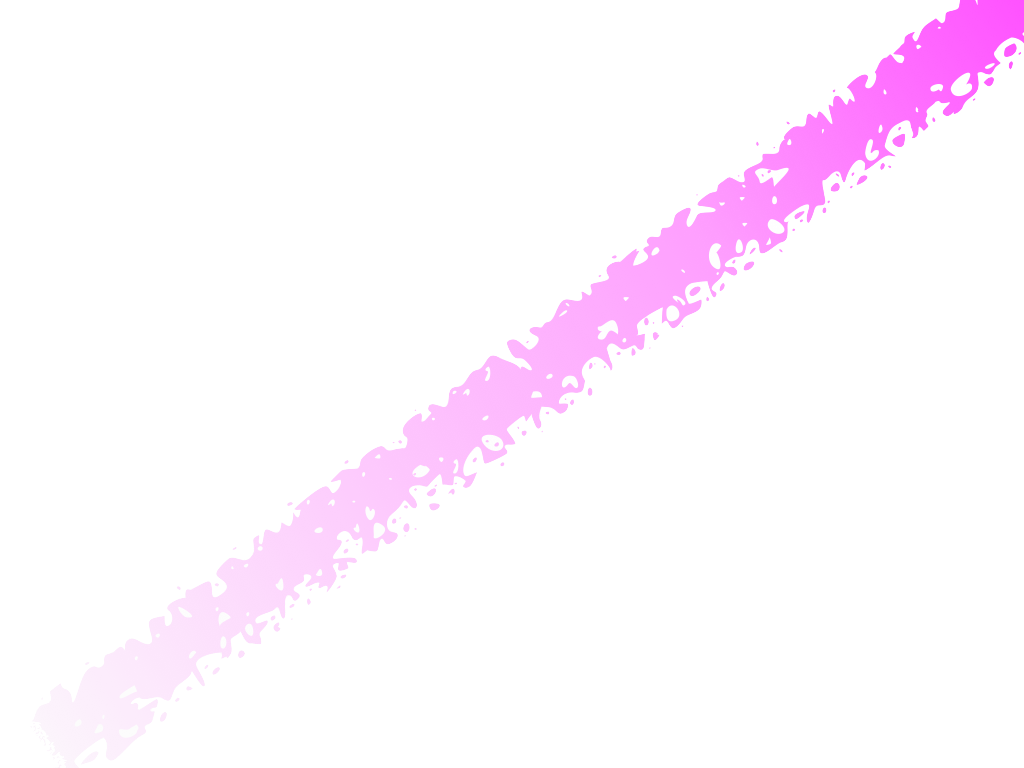
\includegraphics[width=0.20\textwidth]{images/model_components_cartoons_008} \\
\begin{spacing}{1.0}
\raggedright{\small
\textbf{Role Switching} occurs 1cm from food (forager $\rightarrow$ returner) or nest (returner $\rightarrow$ forager)}
\end{spacing} &
\begin{spacing}{1.0}
\raggedright{\small
\textbf{Pheromone Deposit} rate proportional to ant speed (i.e. uniform per unit distance)}
\end{spacing} &
\begin{spacing}{1.0}
\raggedright{\small
\textbf{Pheromone Response} difference in pheromone between L and R determines magnitude}
\end{spacing} &
\begin{spacing}{1.0}
\raggedright{\small
\textbf{Pheromone Evaporation} rate proportional to pheromone concentration}
\end{spacing} \\[-1.5cm]
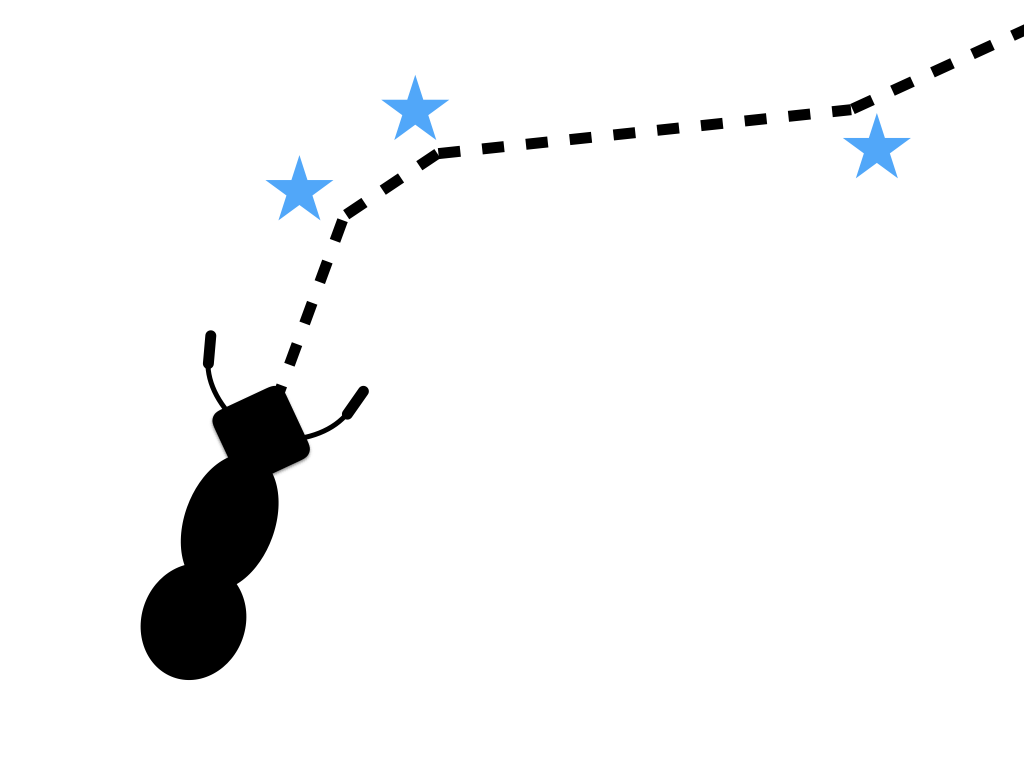
\includegraphics[width=0.20\textwidth]{images/model_components_cartoons_009} &
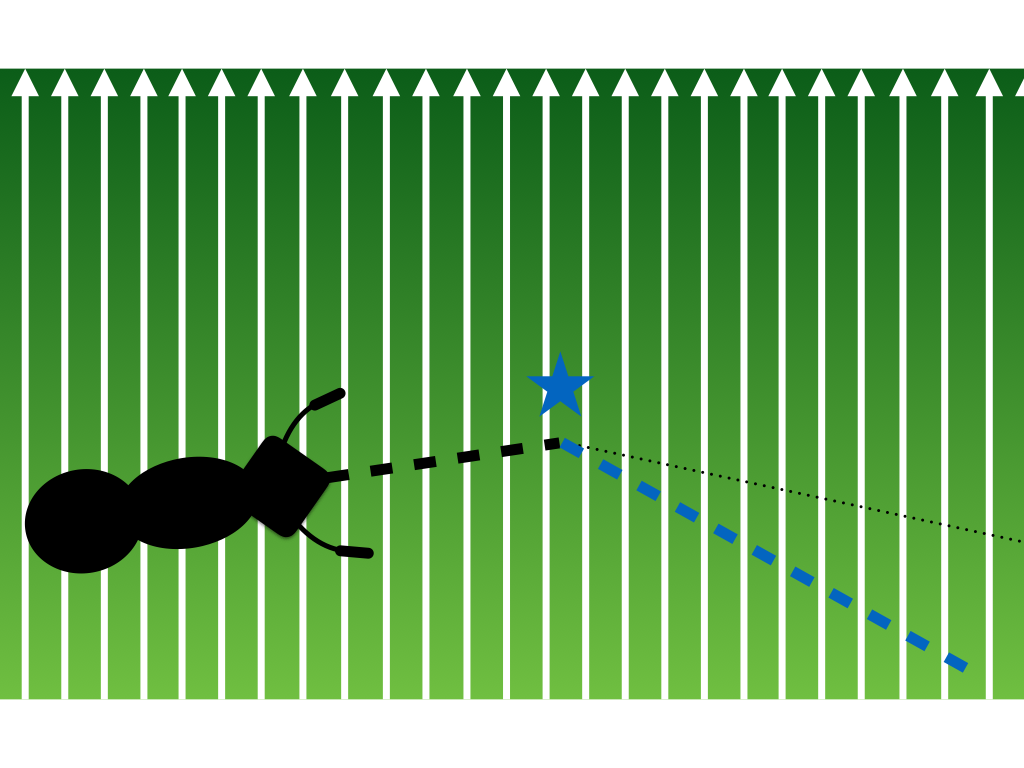
\includegraphics[width=0.20\textwidth]{images/model_components_cartoons_012} &
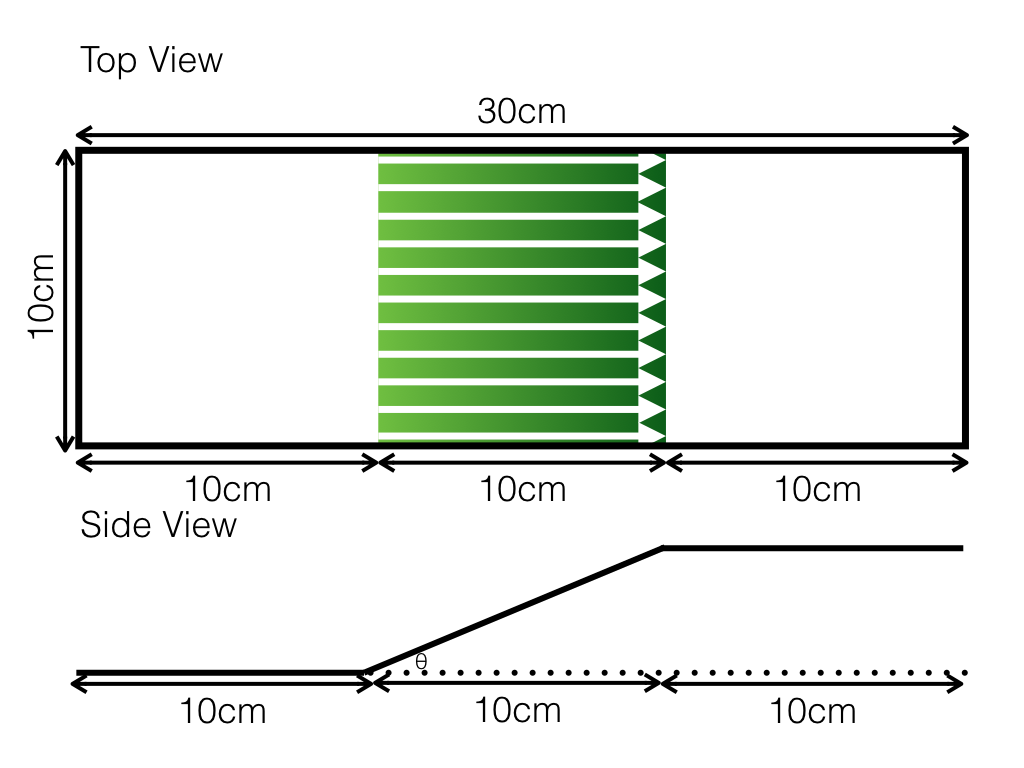
\includegraphics[width=0.20\textwidth]{images/model_components_cartoons_011} &
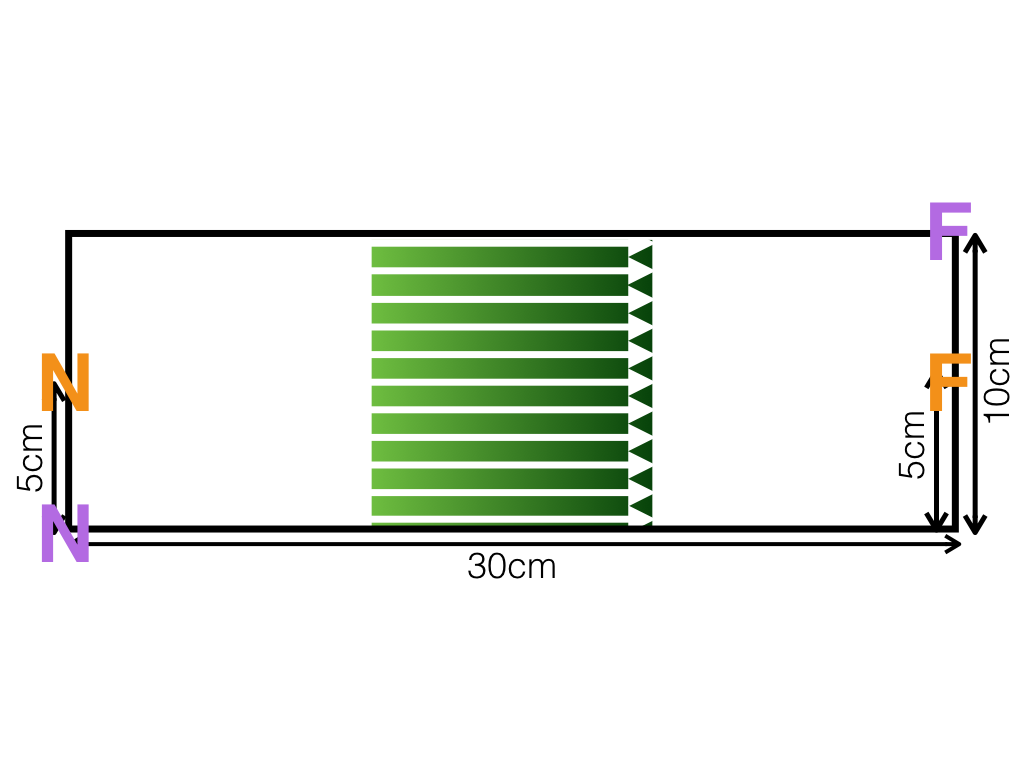
\includegraphics[width=0.20\textwidth]{images/model_components_cartoons_010} \\
\begin{spacing}{1.0}
\raggedright{\small
\textbf{``Boltzmann walker''} ant heading modified at occasional random reorientation events}
\end{spacing} &
\begin{spacing}{1.0}
\raggedright{\small
\textbf{Reorientation on Incline} random reorientation biased to alignments parallel to gradient}
\end{spacing} &
\begin{spacing}{1.0}
\raggedright{\small
\textbf{Arena Terrain} comprised of two flat sections joined by a simple incline}
\end{spacing} &
\begin{spacing}{1.0}
\raggedright{\small
\textbf{Nest/Food Placement} center-to-center shown in orange, corner-to-corner shown in purple}
\end{spacing} \\
\end{tabular}
\end{block} 

%----------------------------------------------------------------------------------------
\vspace{-6ex}
\begin{columns}[t,totalwidth=\twocolwid] % Split up the two columns wide column again

\begin{column}{\onecolwid} % The first column within column 2 (column 2.1)

%----------------------------------------------------------------------------------------
%	MATHEMATICAL SECTION
%----------------------------------------------------------------------------------------

% \begin{block}{Arena Schematics}
% \vspace{-2ex}
% \begin{columns}[T,onlytextwidth]
% \column{0.45\textwidth}

% \begin{figure}
%     	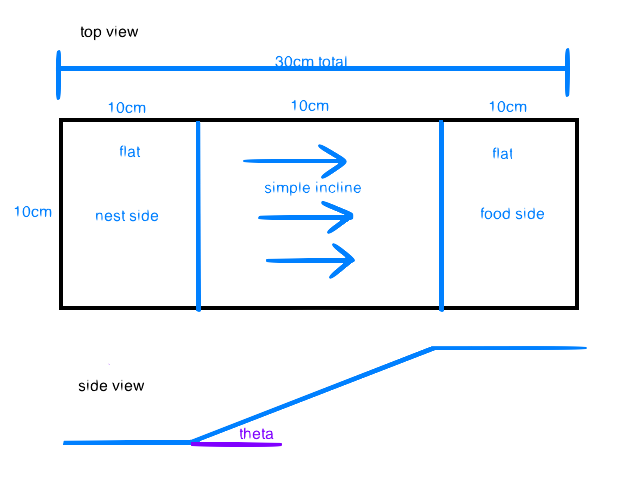
\includegraphics[width=0.8\textwidth]{images/simple_incline_schematic}
%         \begin{spacing}{1.0}
%         \caption{Arena terrain scheme}
%         \end{spacing}
%  \end{figure}
%  \column{0.1\textwidth}
%  \column{0.45\textwidth}
%   \begin{figure}
%   \begin{tabular}{ll}
%     {\scriptsize \begin{tabular} center-to-center \\ arena \end{tabular}}	& \raisebox{-.5\height}{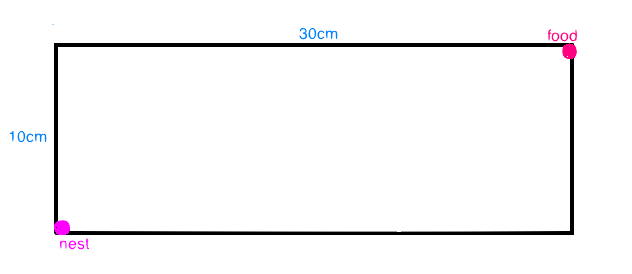
\includegraphics[width=0.6\textwidth]{images/cross_food_schematic}}\\
%    {\scriptsize \begin{tabular} corner-to-corner \\ arena \end{tabular}}  & \raisebox{-.5\height}{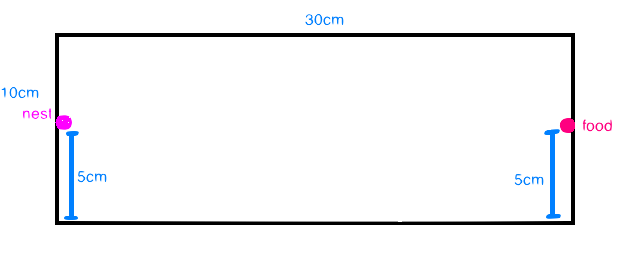
\includegraphics[width=0.6\textwidth]{images/middle_food_schematic}}
%    \end{tabular}
%    \begin{spacing}{1.0}
%    \caption{Nest and food placement scheme}
%    \end{spacing}
%   \end{figure}
% \end{columns}
% \end{block}


%----------------------------------------------------------------------------------------

\end{column} % End of column 2.1

\begin{column}{\onecolwid} % The second column within column 2 (column 2.2)


\end{column} % End of column 2.2

\end{columns} % End of the split of column 2

\end{column} % End of the second column

\begin{column}{\sepwid}\end{column} % Empty spacer column

\begin{column}{\onecolwid} % The third column
\vspace{-3.5ex}
\begin{block}{Conclusion}
\vspace{-2.5ex}
\small{
Duration of foraging trips was found to increase with the severity of incline traversed, with uphill foraging trips taking longer than downhill ones. It was also found that foraging paths that traverse severe inclines, both uphill and downhill, tend to be more direct, more stable, and more tightly constrained than foraging paths that traverse gentle inclines or no incline. These effects were observed in the corner-to-corner setup, where the direct path crosses the incline at an angle, and--to a lesser degree--in the center-to-center setup, where the direct path is aligned with the incline.
}
\end{block}


%----------------------------------------------------------------------------------------
%	REFERENCES
%----------------------------------------------------------------------------------------
\vspace{-3ex}
\begin{block}{References}
\vspace{-2.5ex}
\nocite{*} % Insert publications even if they are not cited in the poster
{\tiny\bibliographystyle{abbrv}
\bibliography{mbi_reu_bib}}
\end{block}

%----------------------------------------------------------------------------------------
%	ACKNOWLEDGEMENTS
%----------------------------------------------------------------------------------------
\vspace{-3.5ex}

\begin{block}{Acknowledgements}
\vspace{-2.5ex}
\begin{spacing}{1.0}
\scriptsize{\rmfamily{I am grateful for the excellent mentorship of Jason Graham and Simon Garnier. Thanks to the New Jersey Institute of Technology and the Ohio State University for hosting me this summer, as well as the Mathematical Biosciences Institute for coordinating this program. I am also grateful to my advisors and mentors at the University of Puget Sound. This material is based upon work supported by the National Science Foundation under Grant No. 1461163.}}
\end{spacing}
\end{block}


\end{column} % End of the third column

\end{columns} % End of all the columns in the poster
\vspace{-1ex}
\deemph{
\noindent\makebox[\paperwidth]{\rule{1.1\paperwidth}{5pt}}}
\vspace{-3.5ex}
\begin{block}{Results}
\vspace{-3.5ex}
\begin{centering}
\begin{tabular}{p{0.42\textwidth} *{4}{|p{0.145\textwidth}}}
\raisebox{-.1\height}{\begin{tabular}{*{3}{p{0.14\textwidth}}}
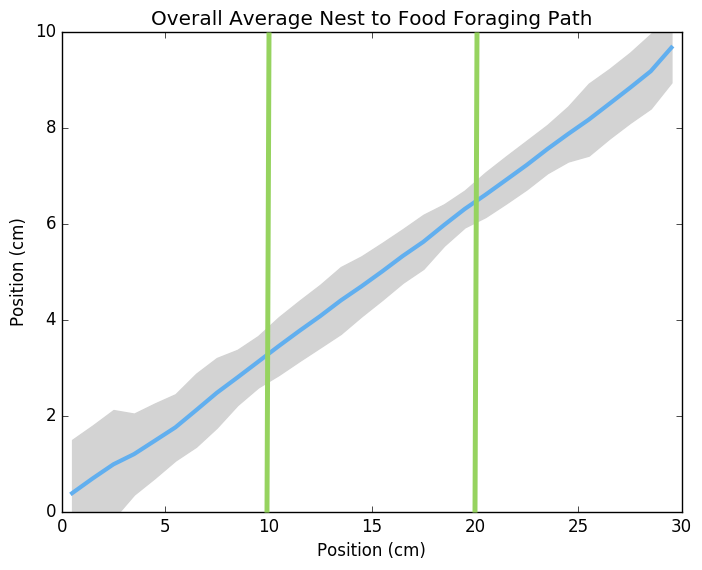
\includegraphics[width=0.12\textwidth]{results/corner-to-corner-average_path_negpidiv3} 
&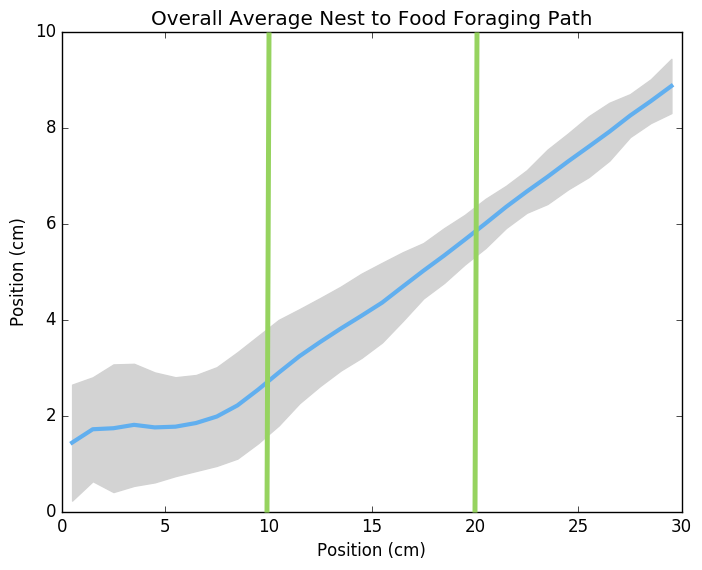
\includegraphics[width=0.12\textwidth]{results/corner-to-corner-average_path_0}
&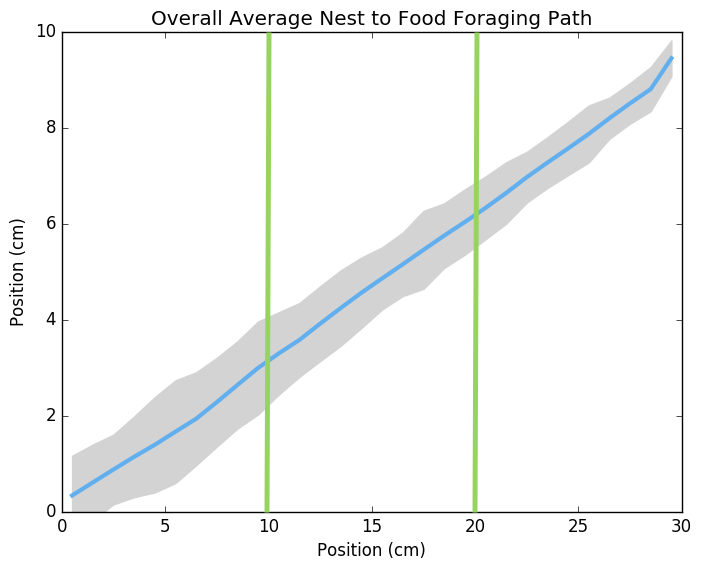
\includegraphics[width=0.12\textwidth]{results/corner-to-corner-average_path_pidiv3}
\end{tabular}}
& \raisebox{-.5\height}{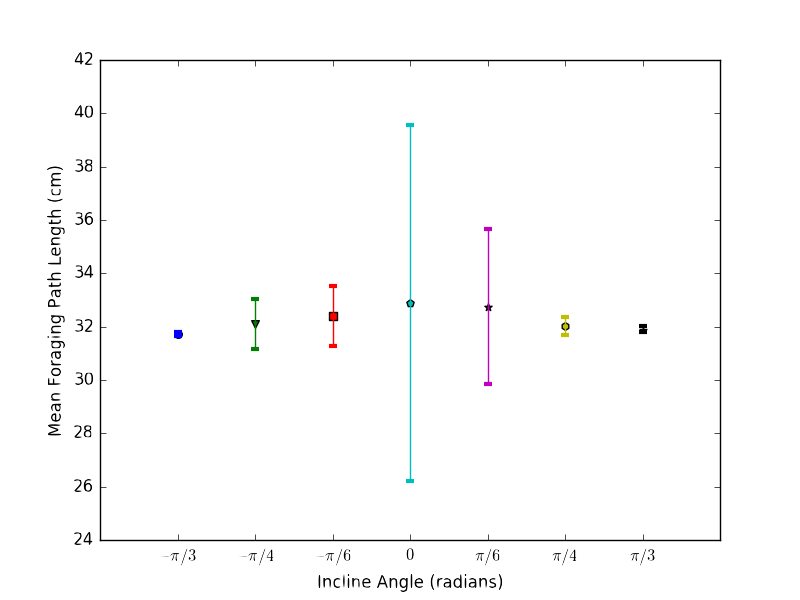
\includegraphics[width=0.14\textwidth]{results/corner-to-cornermeanforagingpathlength}} 
& \raisebox{-.5\height}{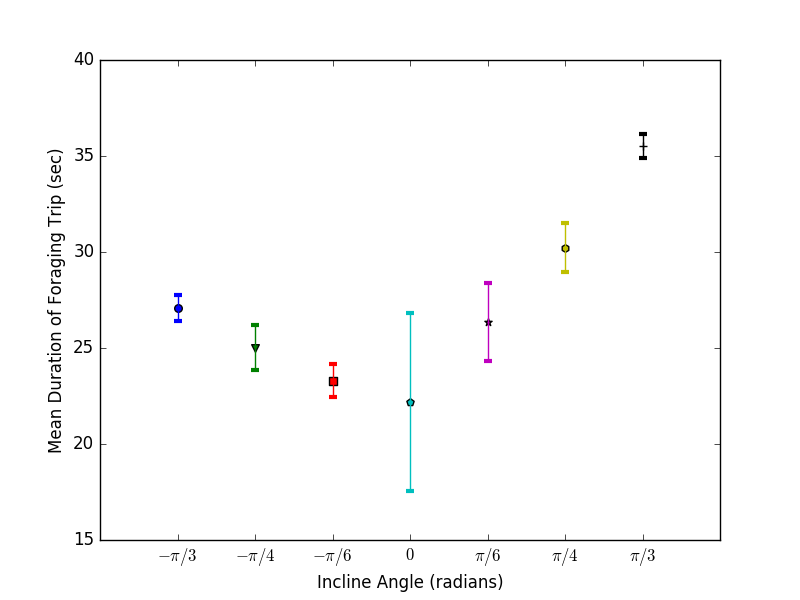
\includegraphics[width=0.14\textwidth]{results/corner-to-cornermeandurationofforagingtrip}} 
& \raisebox{-.5\height}{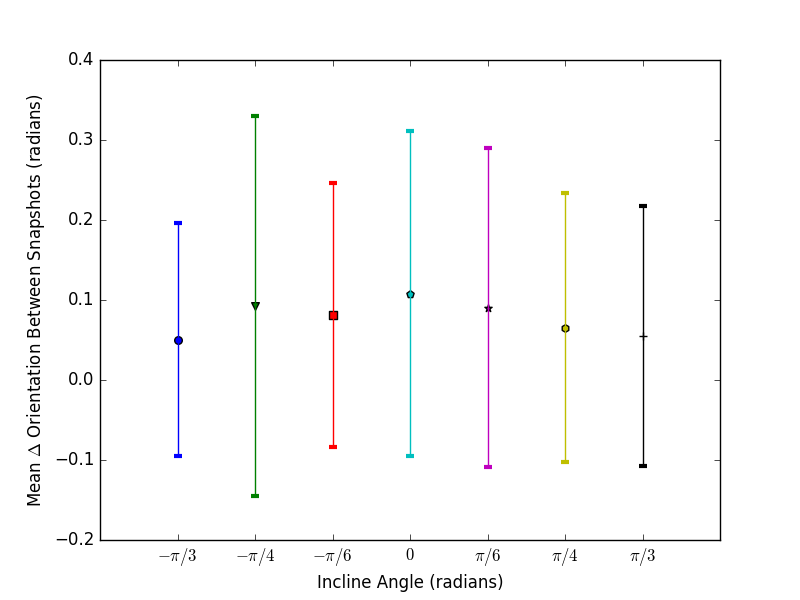
\includegraphics[width=0.14\textwidth]{results/corner-to-corner_meandeltaorientationbetweensnapshots}} 
& \raisebox{-.5\height}{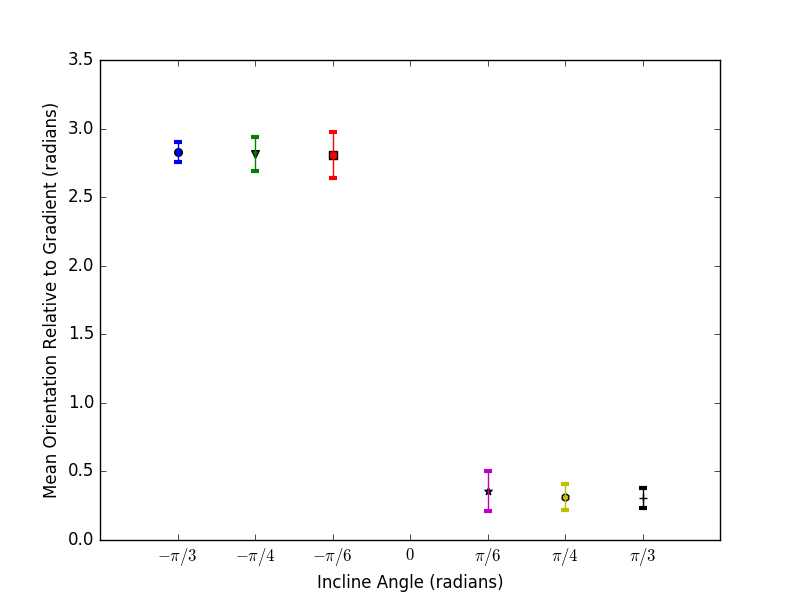
\includegraphics[width=0.14\textwidth]{results/corner-to-cornermeanorientationrelativetogradient}}
\\
\raisebox{-.1\height}{\begin{tabular}{*{3}{p{0.14\textwidth}}}
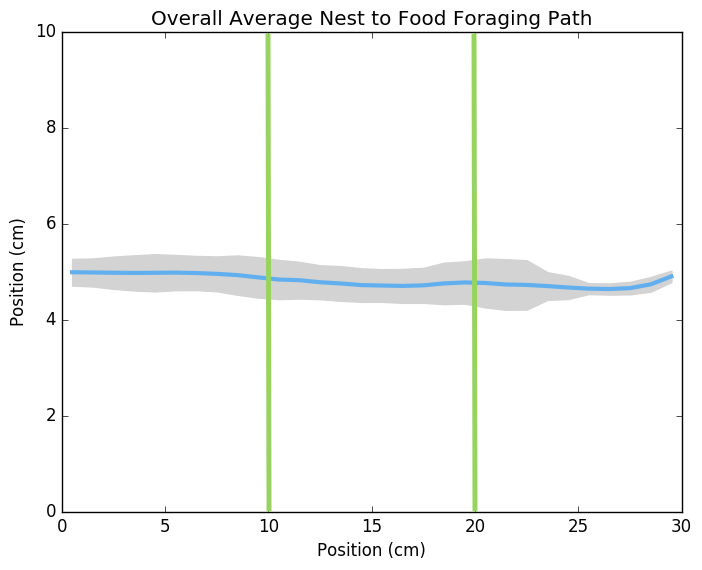
\includegraphics[width=0.12\textwidth]{results/center-to-center-average_path_negpidiv3.png}
& 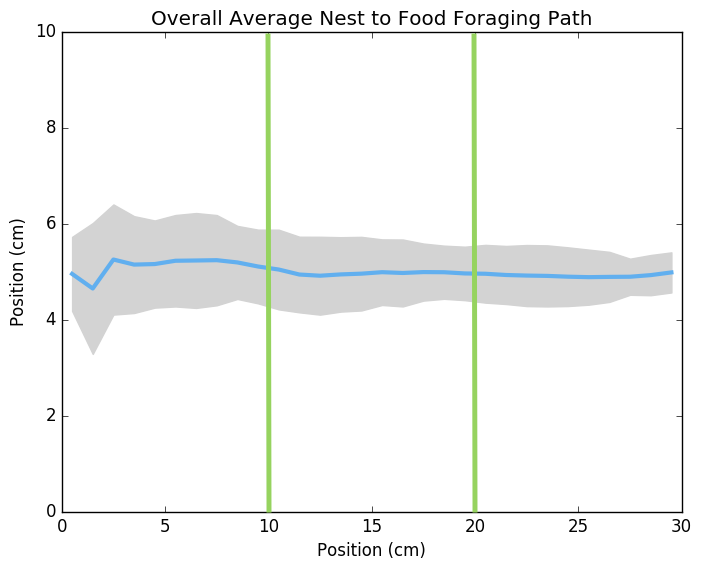
\includegraphics[width=0.12\textwidth]{results/center-to-center-average_path_0.png}
& 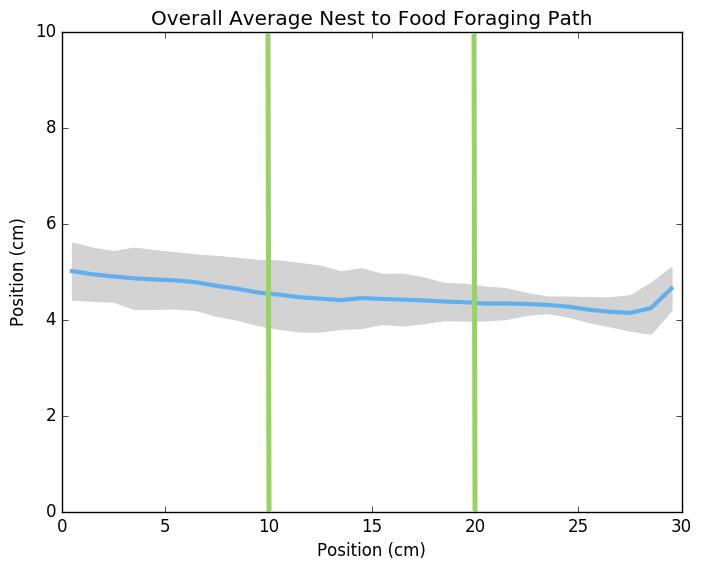
\includegraphics[width=0.12\textwidth]{results/center-to-center-average_path_pidiv3.png}
\end{tabular}}
& \raisebox{-.5\height}{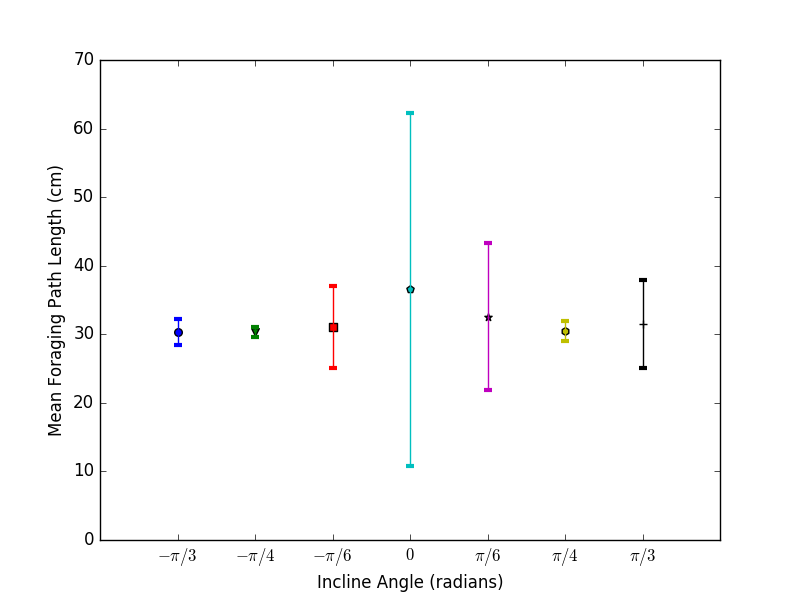
\includegraphics[width=0.14\textwidth]{results/center-to-centermeanforagingpathlength.png}} 
& \raisebox{-.5\height}{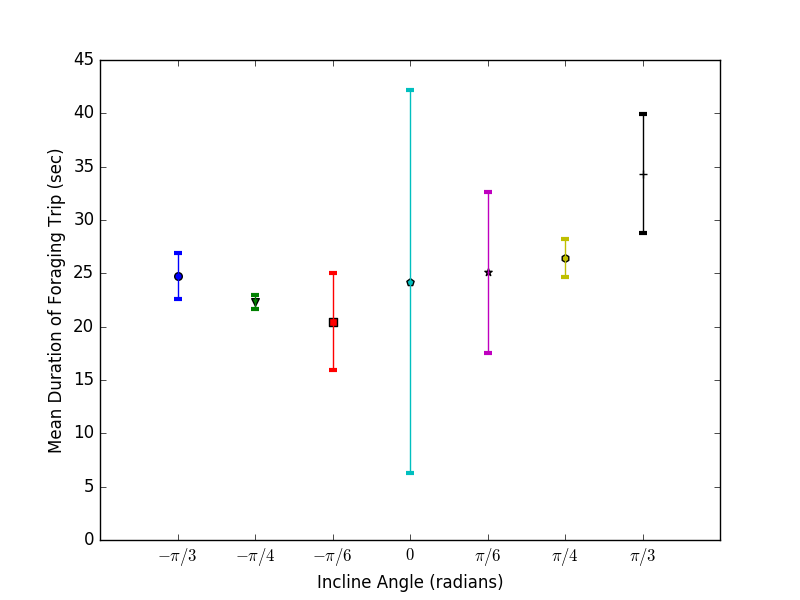
\includegraphics[width=0.14\textwidth]{results/center-to-centermeandurationofforagingtrip.png}} 
& \raisebox{-.5\height}{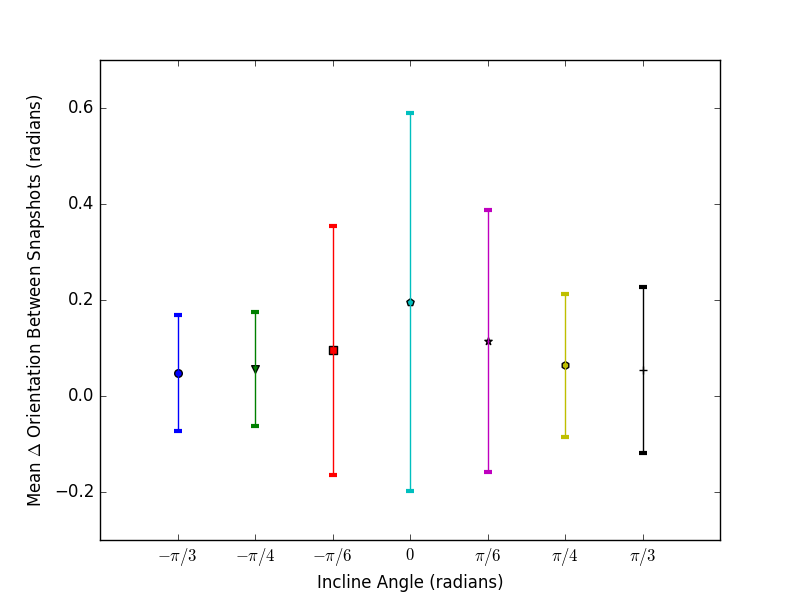
\includegraphics[width=0.14\textwidth]{results/center-to-center_meandeltaorientationbetweensnapshots.png}} 
& \raisebox{-.5\height}{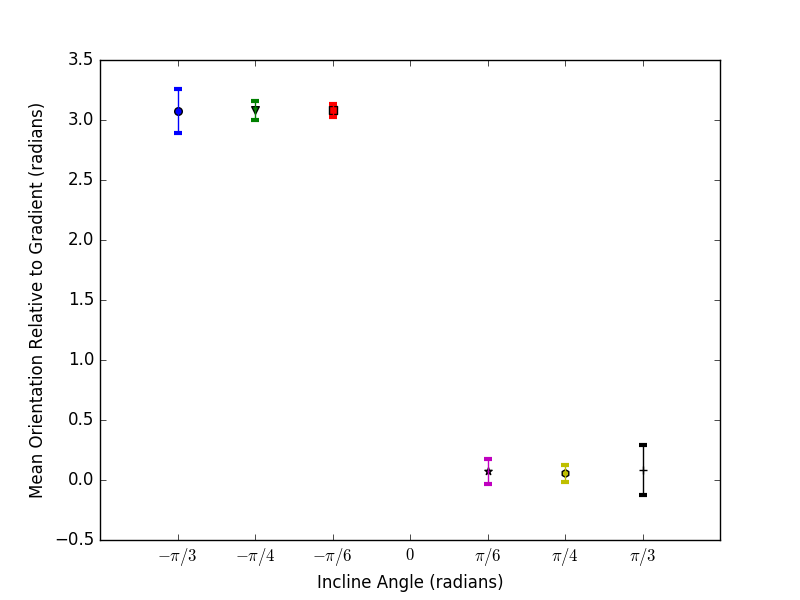
\includegraphics[width=0.14\textwidth]{results/center-to-centermeanorientationrelativetogradient.png}} 
 \\
 \begin{spacing}{1.0}
 \footnotesize{
Comparison of overall average nest to food foraging path for, left to right, $-\pi/3$, $0$, and $\pi/3$ radian inclines on corner-to-corner arenas (top) and center-to-center arenas (bottom). The blue line indicates the mean path and the gray shading indicates the magnitude of one standard deviation at each x value.}
\end{spacing}
& 
\begin{spacing}{1.0}
\footnotesize{
Comparison of nest-to-food path lengths over several incline angles; corner-to-corner arena top and center-to-center arena bottom.
}
\end{spacing}
&
\begin{spacing}{1.0}
\footnotesize{
Comparison of nest-to-food trip durations over several incline angles; corner-to-corner arena top and center-to-center arena bottom.}
\end{spacing}
&
\begin{spacing}{1.0}
\footnotesize{
Comparison of changes in heading over half second intervals during nest-to-food travel over several incline angles; corner-to-corner arena top and center-to-center arena bottom.
}
\end{spacing}
& 
\begin{spacing}{1.0}
\footnotesize{
Comparison of orientation relative to gradient over incline angles; a direct path would be oriented at 2.82/0.32 radians for the corner-to-corner arena (top) and at 0/3.14 radians for the center-to-center arena (bottom).}
\end{spacing}
\end{tabular}
\end{centering}
\end{block}
   
%    \begin{block}{Results: Path Shape}
% \begin{figure}

% % incline & corner-to-corner & center-to-center \\
% % $-\pi/3$ &  &  \\
% % $0$ &  &   \\
% % $\pi/3$ & &   \\
% % \end{tabular}
% \begin{spacing}{1.0}
% \caption{}
% \end{spacing}
% \end{figure}
% \end{block}
    

\end{frame} % End of the enclosing frame

\end{document}
